\chapter{Auswertung}
\section{Kapazität des variablen Kondensators}
Durch \gl{eq:c1} lässt sich die Kapazität $ C_{1} $ des Kondensators in Abhängigkeit der Kapazität des Vergleichskondensators $ C_{2}=\SI{220}{nF}$
und den beiden Spannungen $ U_1 $ und $ U_2(d) $
der Messtabelle \tabelle{tab:mess1} berechnen.\par
\gl{eq:plattencap} gibt uns den eigentlich berechneten Wert der Kapazität $ C_{1} $ mit $\varepsilon_{0}=\SI{8,854}{\cdot 10^{-12}\frac{As}{Vm}}$,
$ \varepsilon_{R,Luft}=1 $ und $ D=\SI{0,255}{m} $ für $ \SI{1}{mm} \leq d \leq \SI{10}{mm} $.\par
Trägt man die drei experimentell bestimmten Kapazitäten zusammen mit der berechneten als Funktion des Abstandes auf, so erhält man
folgendes Diagramm:\par
\begin{figure}[h]
    \centering
    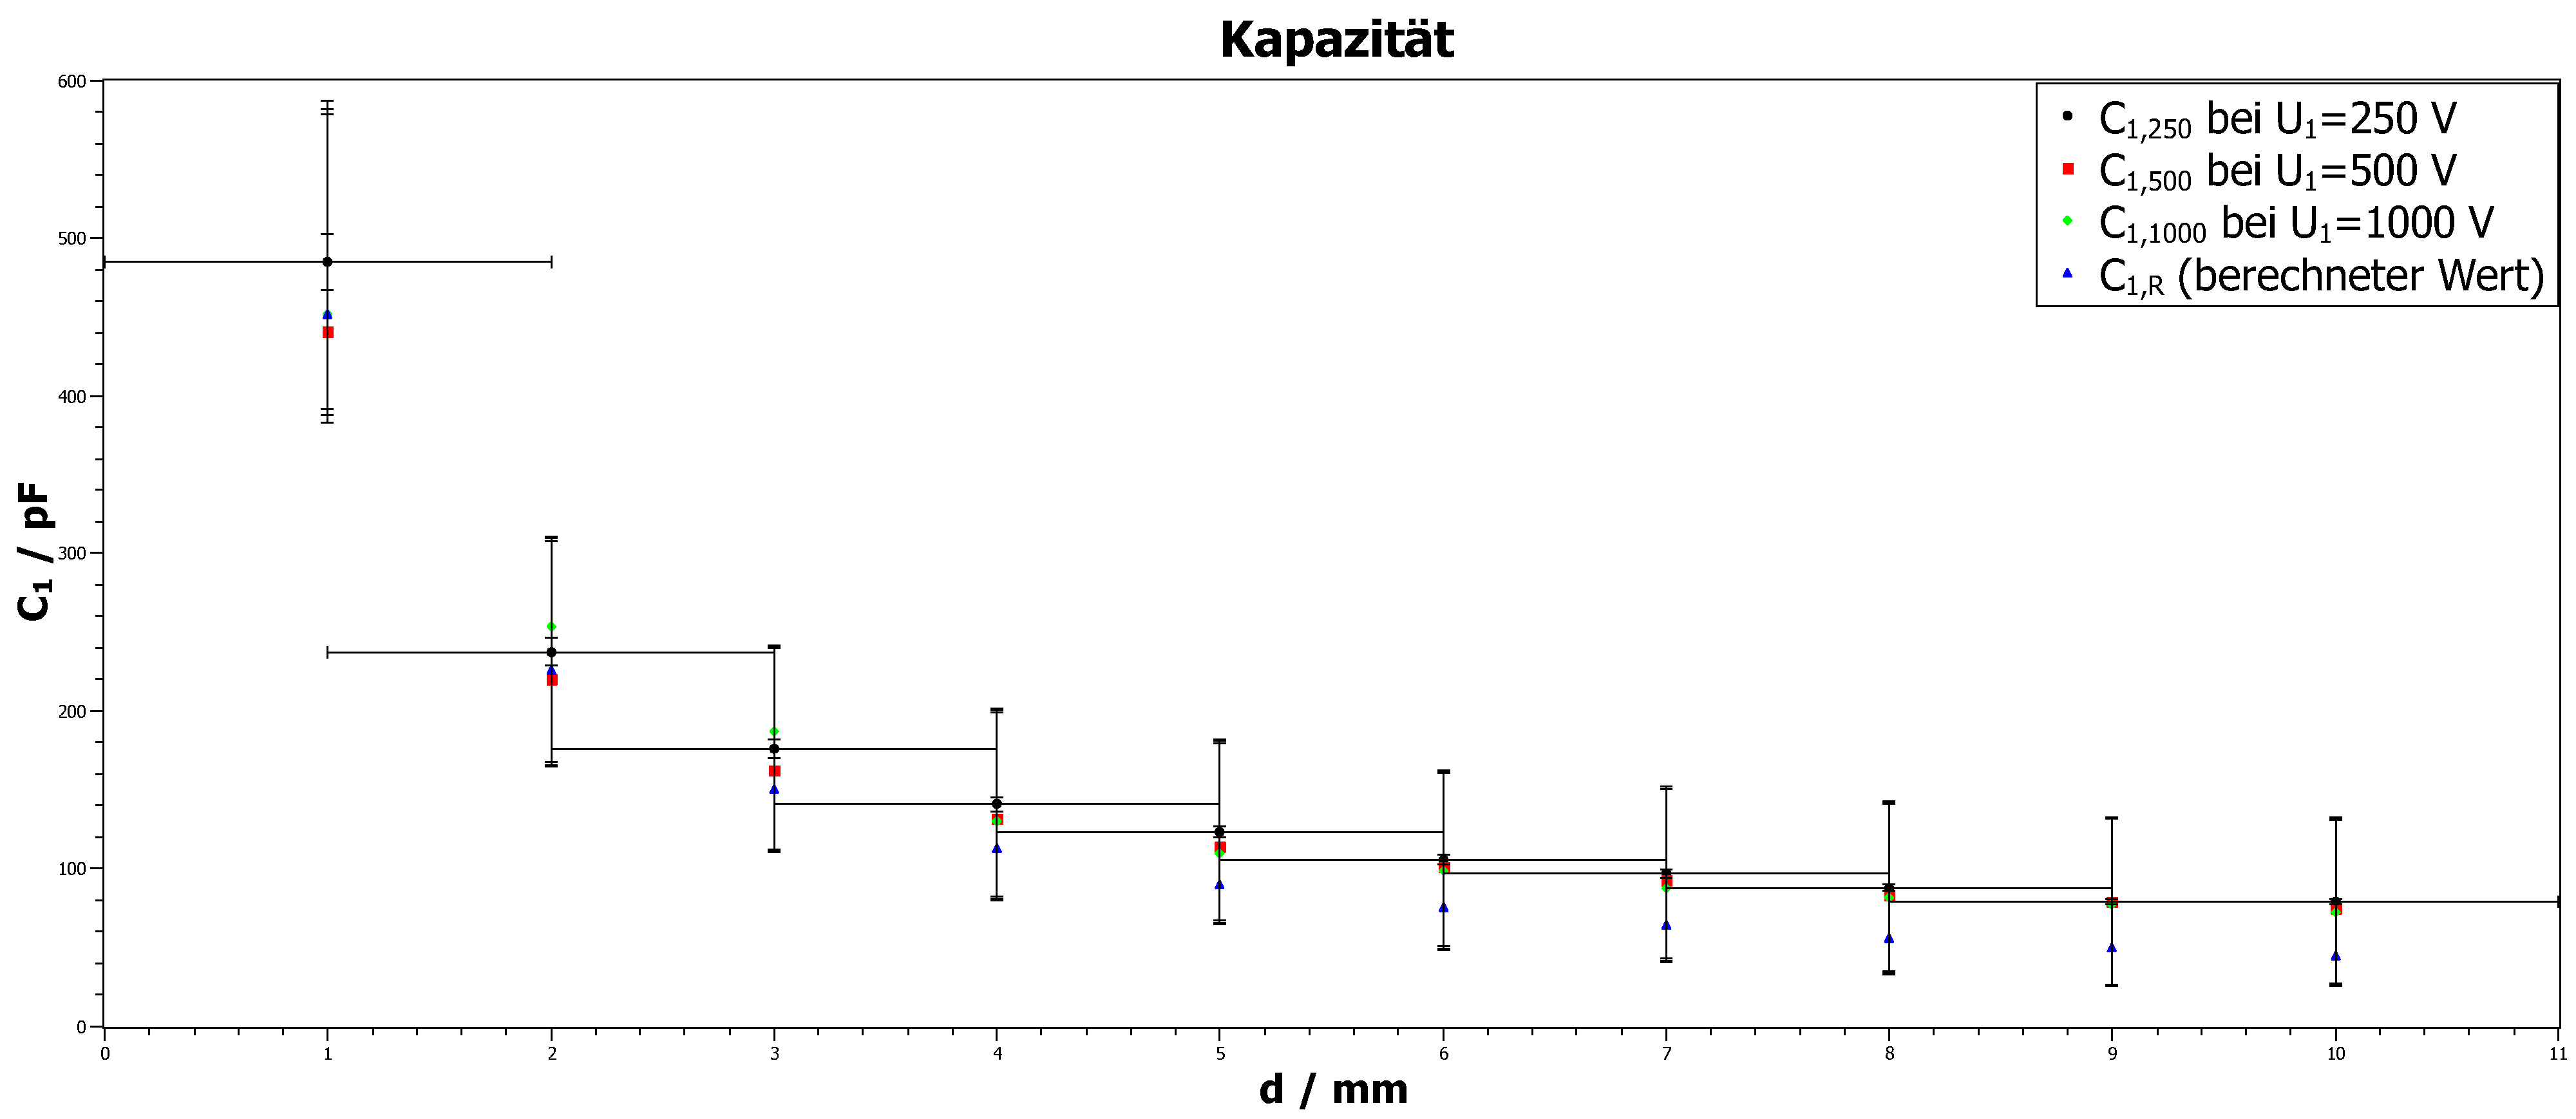
\includegraphics[width=.95\textwidth]{diagramme/Kapazitaet.pdf}
    \caption[Diagram Kapazität]{Diagram Kapazität}
    \label{fig:farad}
\end{figure}
%
\subsection{Fehler der experimentell bestimmten Kapazität}
Für den Fehler der experimentell bestimmten Kapazitäten gilt:
\begin{align}
    C_{1} &= C_{2}\cdot \left(\frac{U_{1}}{U_{2}}-1\right)^{-1} \nonumber \\
    \Delta C_{1} &= \left\vert\frac{\partial C_{1}}{\partial C_{2}}\right\vert\cdot \Delta C_{2} + \left\vert\frac{\partial C_{1}}{\partial U_{1}}\right\vert\cdot \Delta U_{1} + \left\vert\frac{\partial C_{1}}{\partial U_{2}}\right\vert\cdot \Delta U_{2} \nonumber \\
    &= \left(\frac{U_{1}}{U_{2}}-1\right)^{-1}\cdot \Delta C_{2} + C_{2}\cdot\left(\frac{U_{1}}{U_{2}}-1\right)^{-2}\cdot \frac{1}{U_{2}}\cdot\Delta U_{1} + C_{2}\cdot\left(\frac{U_{1}}{U_{2}}-1\right)^{-2}\cdot \frac{U_{1}}{U_{2}^{2}}\cdot\Delta U_{2}
\end{align}
Für den Fehler der berechneten Kapazität gilt:
\begin{align}
    C_{1,R} &= \varepsilon_{0} \varepsilon_{R} \cdot \frac{D^{2} \pi}{4 d} \nonumber \\
    \Delta C_{1,R} &= \left\vert\frac{\partial C_{1,R}}{\partial D}\right\vert\cdot \Delta D + \left\vert\frac{\partial C_{1,R}}{\partial d}\right\vert\cdot \Delta d \nonumber \\
    &= \varepsilon_{0}\varepsilon_{R}\cdot\frac{D \pi}{2 d}\cdot \Delta D + \varepsilon_{0} \varepsilon_{R}\cdot\frac{D^{2} \pi}{4 d^{2}}\cdot \Delta d
\end{align}
mit $ \Delta D= \SI{0,005}{m} $
%
%
%
\section{Bestimmung der elektrischen Feldkonstante}
Über die Steigung $ m $ der Ausgleichsgeraden der Funktion $ C_{1}(d^{-1}) $ lässt sich mittels \gl{eq:e0} die
elektrische Feldkonstante $\varepsilon_0$ bestimmen. Wird $ C_{1,\SI{1000}{V}} $ über $ d^{-1} $ aufgetragen ergibt sich
der in \bild{fig:mu_0} zu sehende Verlauf\par
\begin{figure}[h]
    \centering
    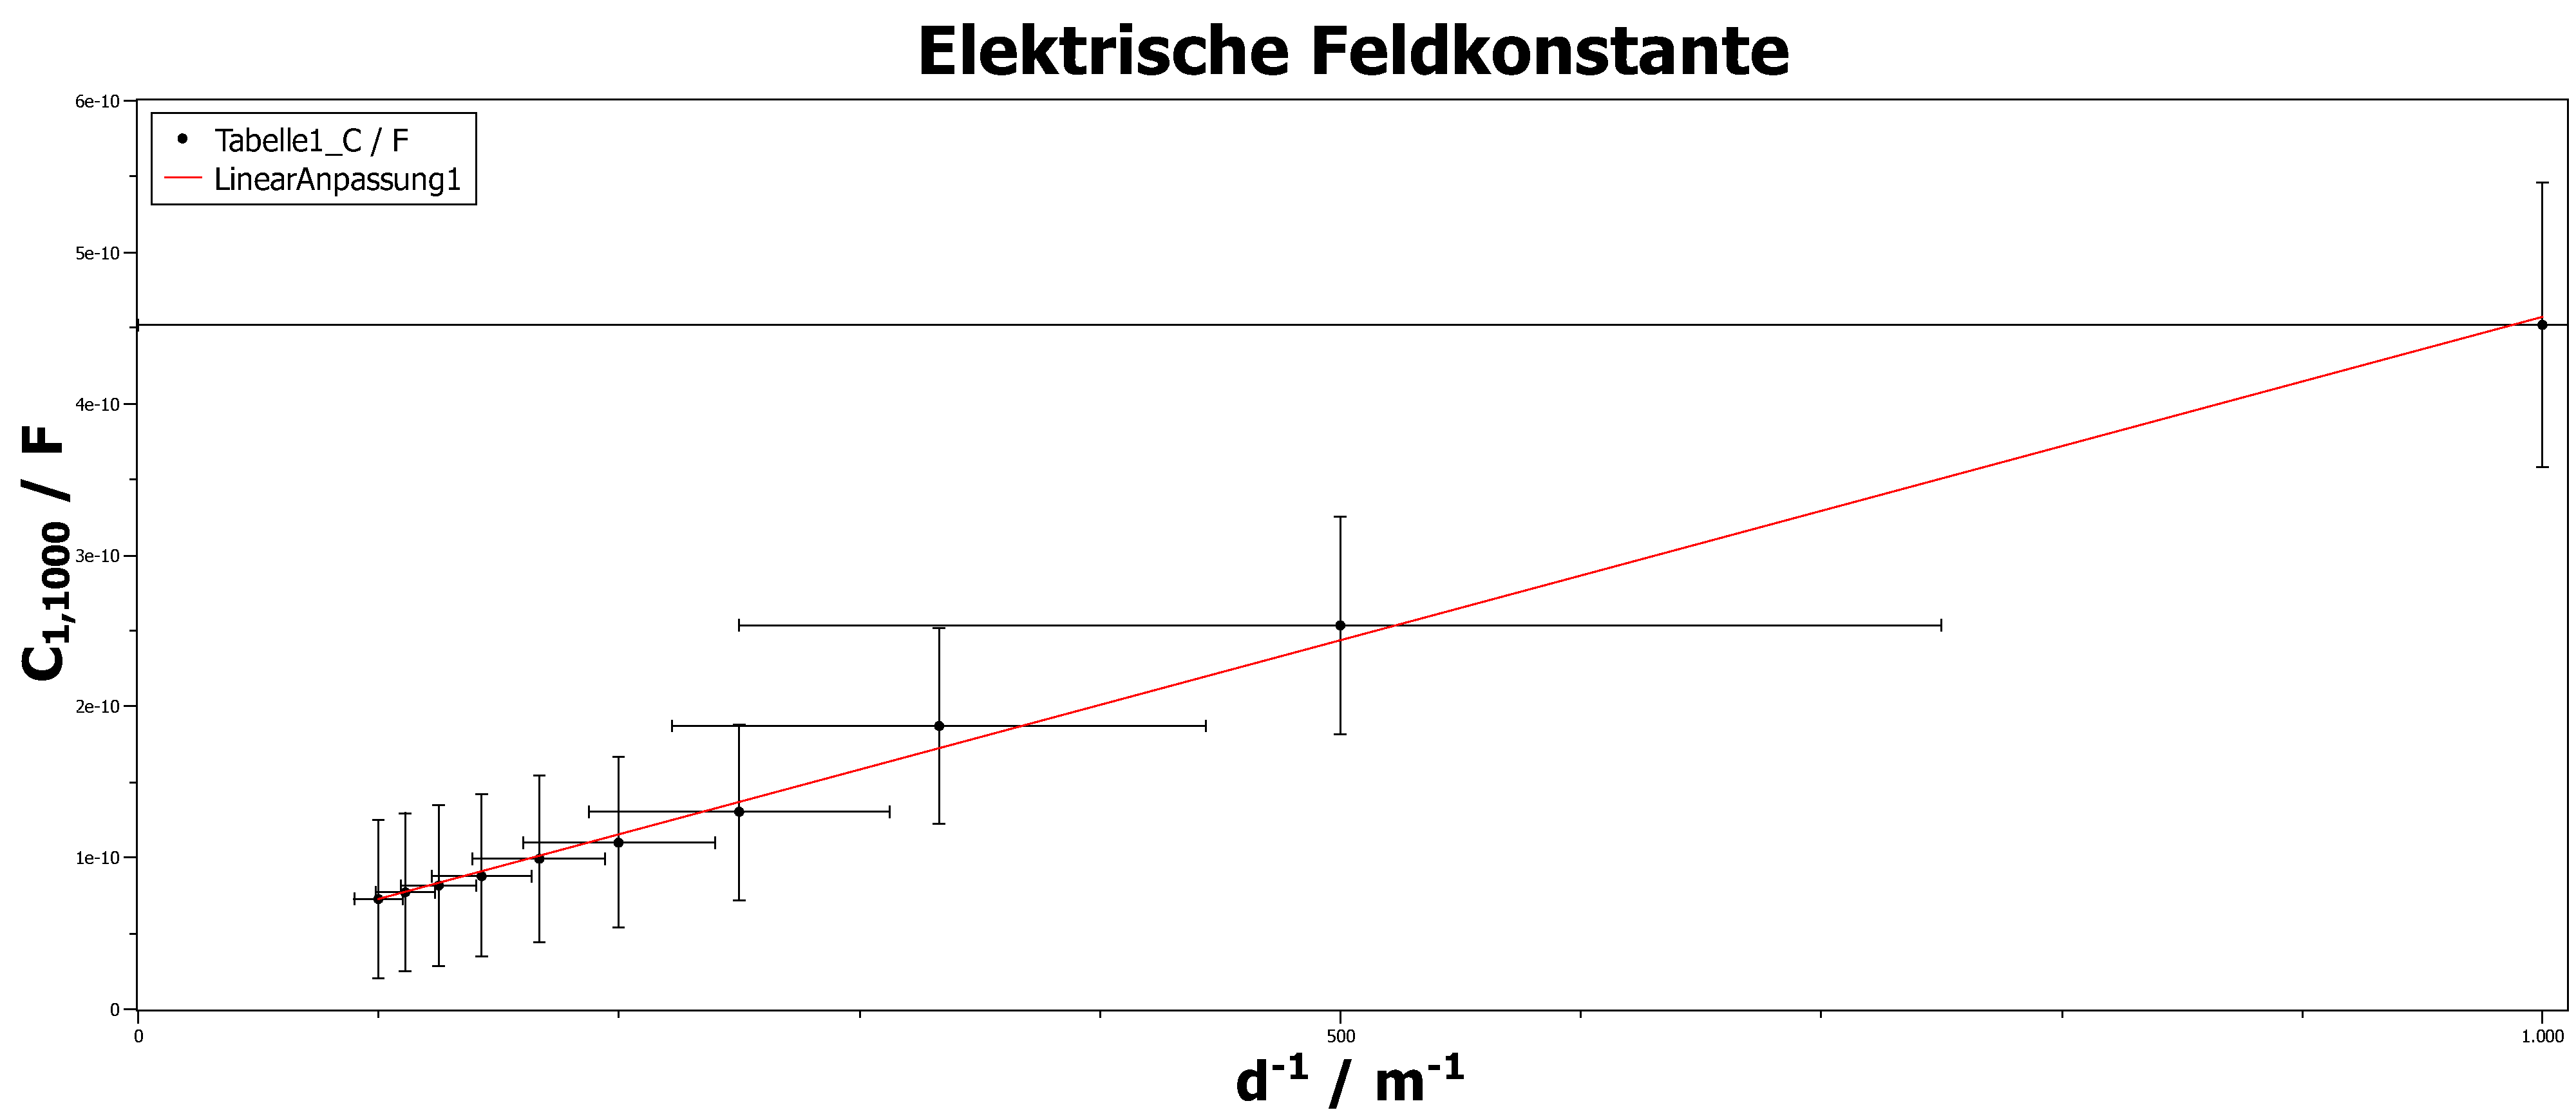
\includegraphics[width=.95\textwidth]{diagramme/Elektrische_Feldkonstante.pdf}
    \caption[Diagram elektrische Feldkonstante]{Diagram elektrische Feldkonstante}
    \label{fig:mu_0}
\end{figure}
%
mit der durch \textit{SciDAVis} ermittelten Steigung der Ausgleichsgeraden von:
%
\begin{align}
    m=(4,3 \pm 0,7){\cdot 10^{-13}\frac{\text{As}\cdot \text{m}}{\text{V}}}
\end{align}
Für die elektrische Feldkonstante $\varepsilon_{0}$ gilt also:
\begin{align}
    \varepsilon_{0} &= \frac{m}{\varepsilon_{R}\cdot A} \nonumber \\
    &= \frac{4,3\SI{}{\cdot 10^{-13} \frac{As \cdot m}{V}}}{ \frac{\pi}{4} \cdot (\SI{0,255}{m})^{2} } \nonumber \\
    &= 8,420\SI{}{\cdot 10^{-12}\frac{As}{Vm}}
\end{align}
%
\subsection{Fehler der experimentell bestimmten elektrischen Feldkonstante}
Der Fehler der elektrischen Feldkonstante hängt von der Abweichung der Steigung und des Durchmessers ab. So gilt:
\begin{align}
    \varepsilon_{0} &= \frac{4 m}{D^{2} \pi} \nonumber \\
    \Delta\varepsilon_{0} &= \left\vert\frac{\partial\varepsilon_{0}}{\partial m}\right\vert \cdot \Delta m + \left\vert\frac{\partial\varepsilon_{0}}{\partial D}\right\vert \cdot \Delta D \nonumber \\
    &= \frac{4}{D^2 \pi} \cdot \Delta m + \frac{8 m}{D^3 \pi} \cdot \Delta D \nonumber \\
    &= \frac{4}{(\SI{0,255}{m})^{2} \cdot \pi} \cdot \SI{0,7}{\cdot 10^{-13}\frac{As\cdot m}{V}} + \frac{8 \cdot \SI{4,3}{\cdot 10^{-13}\frac{As \cdot m}{V}}}{(\SI{0,255}{m})^{3} \cdot \pi} \cdot \SI{0,005}{m} \nonumber \\
    &= \SI{1,37}{\cdot 10^{-12}\frac{As}{Vm}} + \SI{0,33}{\cdot 10^{-12}\frac{As}{Vm}} \nonumber \\
    &= \SI{1,70}{\cdot 10^{-12}\frac{As}{Vm}}
\end{align}
Ermittelte elektrische Feldkonstante:\par
\begin{align}
    \varepsilon_{0}=(8,4\pm 1,7){\cdot 10^{-12}\frac{\text{As}}{\text{Vm}}}
\end{align}
%
%
%
\section{Bestimmung der Dielektrizitätszahlen}
Über das Verhältnis der beiden Kapazitäten mit und ohne Platte kann nach \gl{eq:rel_feld} die Dielektrizitätszahl
$\varepsilon_{r}$ des jeweiligen Materials bestimmt werden.\par
Zunächst wurden in \textit{SciDAVis} die Spannungen $ U_{2} $, so wie die Kapazitäten $ C_{D} $ und $ C_{0} $ umgerechnet
und abschließend in Relation gesetzt. Die so ermittelten Mittelwerte mit jeweiliger Standardabweichung sind folgende:
\begin{align}
    \varepsilon_{R,Plexiglas} &= 4,05\pm 0,15\\
    \varepsilon_{R,Pertinax} &= 8,73\pm 0,92
\end{align}